\documentclass[14pt, a4paper]{extarticle}
\usepackage{mospolytech_coursework}
\usepackage{float}
\usepackage{makecell}

% Определение данных
\newcommand{\theme}{%
    Разработка веб-приложения для управления ассортиментом и заказами
магазина цифровой электроники%
}
\newcommand{\subject}{Разработка веб-приложений}
\newcommand{\student}{Кузнецов Данила Ростиславович}
\newcommand{\group}{241-327}
\newcommand{\teacher}{Кружалов Алексей Сергеевич}

\begin{document}
\pagestyle{plain}
\setcounter{tocdepth}{2}

% Титульный лист
\include{title}

% Задание
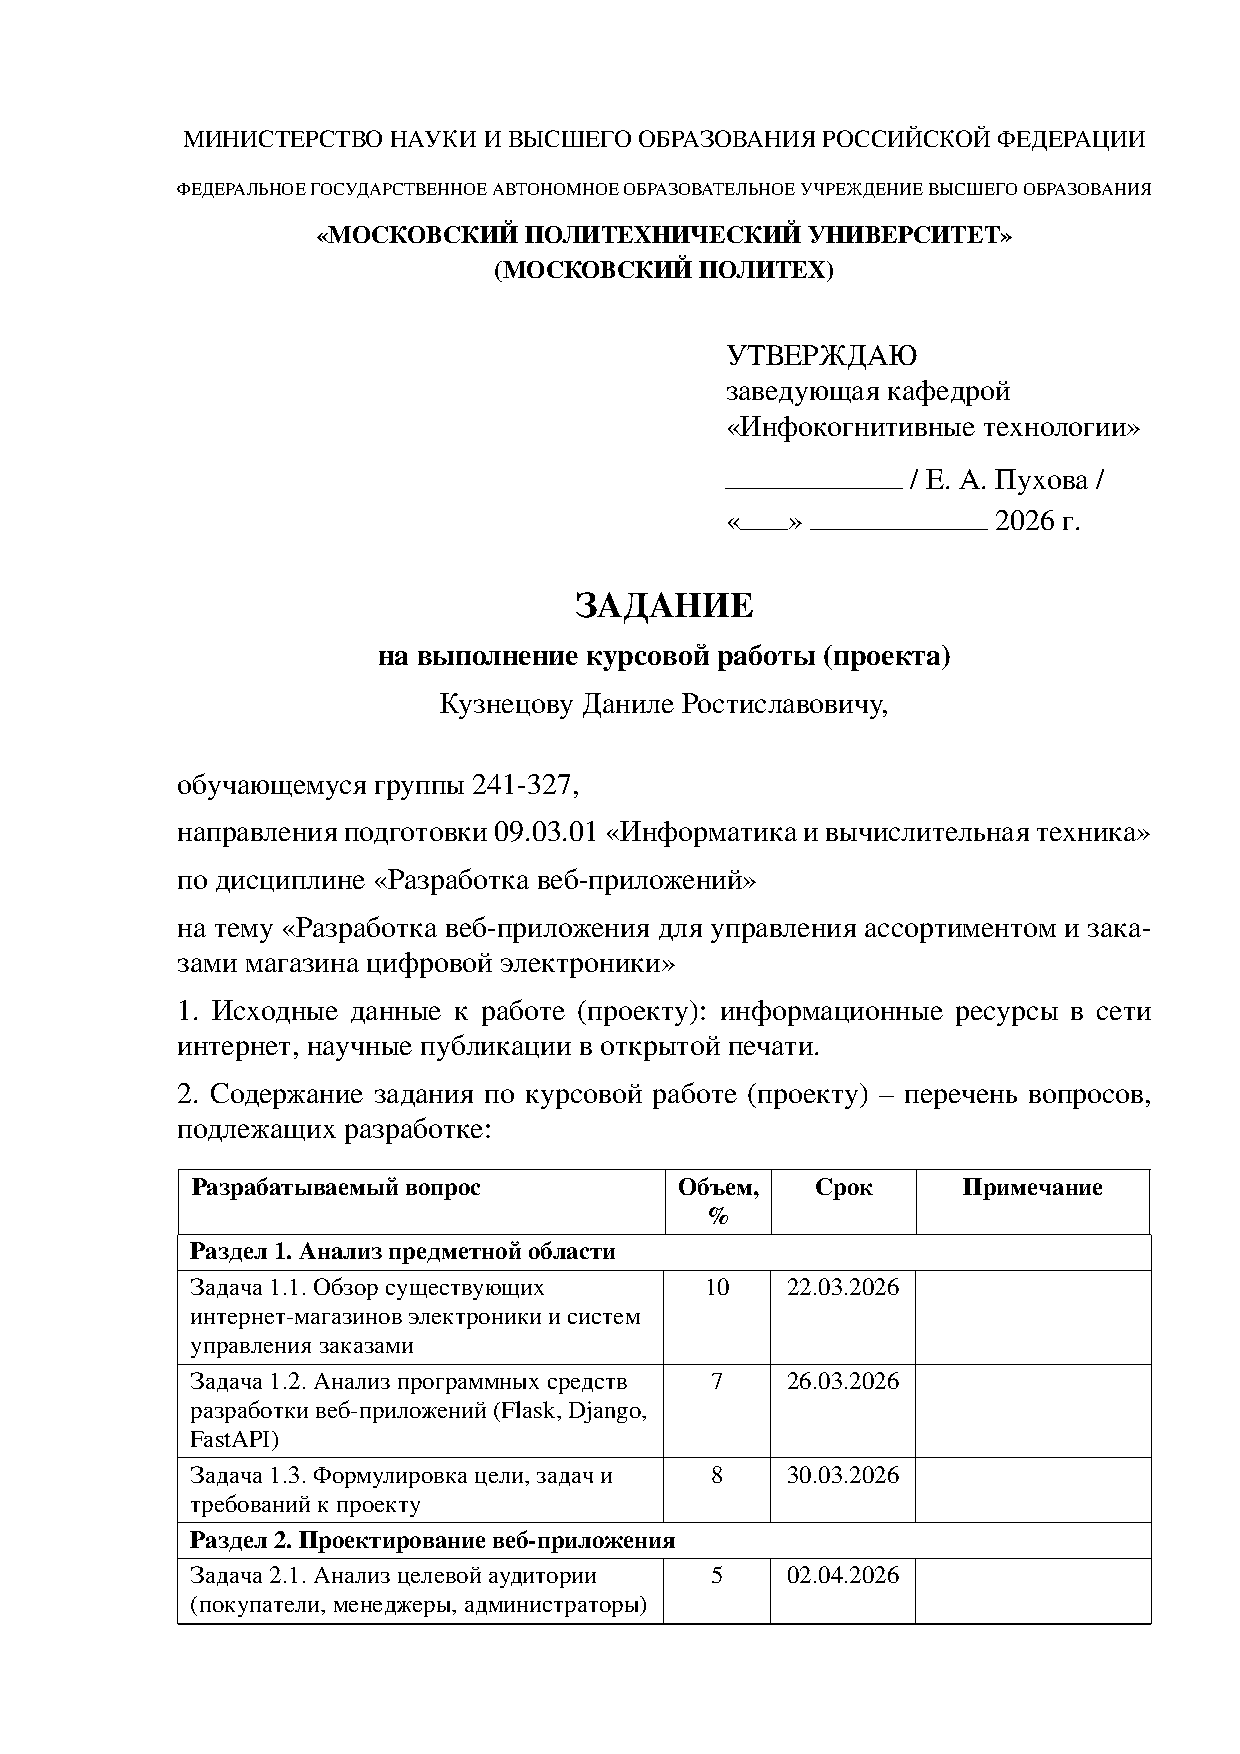
\includepdf[pages=-]{task.pdf}
\clearpage

% Содержание
\tableofcontents


% Введение
\section*{Введение}
\addcontentsline{toc}{section}{Введение}

\textbf{Актуальность темы.} Рынок цифровой электроники характеризуется большим количеством
товарных позиций, быстрым обновлением моделей и высокой зависимостью покупательского выбора
от технических характеристик. Для магазина электроники важно не только представить каталог,
но и обеспечить своевременное обновление цен, остатков, категорий и статусов заказов.
Ручное ведение таких данных увеличивает вероятность ошибок, затрудняет обработку заявок и
снижает качество обслуживания покупателей. Поэтому разработка веб-приложения для управления
ассортиментом и заказами магазина цифровой электроники является актуальной практической задачей.

\textbf{Степень разработанности проблемы.} Современные интернет-магазины и маркетплейсы
предоставляют пользователям развитые средства поиска, фильтрации, оформления заказа и
отслеживания доставки. Однако готовые коммерческие платформы часто ограничивают владельца
магазина правилами конкретной площадки, комиссионной моделью или закрытой логикой управления.
Для небольшого магазина цифровой электроники актуальным остается создание самостоятельного
веб-приложения, которое учитывает особенности ассортимента, роли покупателей, менеджеров и
администраторов, а также требования к обработке заказов.

\textbf{Объект исследования} --- процессы управления онлайн-продажами цифровой электроники,
включая ведение ассортимента, взаимодействие покупателей с каталогом и обработку заказов.

\textbf{Предмет исследования} --- программные средства и архитектурные решения для разработки
веб-приложения, автоматизирующего управление товарами, категориями, пользователями, корзиной
и заказами магазина цифровой электроники.

\textbf{Целью данной работы} является проектирование и реализация веб-приложения для управления
ассортиментом и заказами магазина цифровой электроники, обеспечивающего покупателям удобную
работу с каталогом и заказами, а администраторам --- инструменты управления товарами,
категориями и заявками.


% Основная часть
\clearpage
\section*{Глава 1. Анализ предметной области}
\addcontentsline{toc}{section}{Глава 1. Анализ предметной области}
\stepcounter{section}

\subsection{Обзор существующих интернет-магазинов электроники и систем управления заказами}

Рынок цифровой электроники относится к числу наиболее динамичных сегментов электронной коммерции. Покупатели ожидают от интернет-магазина не только удобного каталога товаров, но и подробных технических характеристик, сравнения моделей, актуальной информации о наличии, понятного оформления заказа, выбора способа доставки и прозрачного отслеживания статуса покупки. Для администрации магазина важны другие задачи: управление ассортиментом, контроль остатков, обработка заказов, обновление цен, работа с категориями, пользователями и историей продаж.

В качестве аналогов были рассмотрены крупные интернет-магазины и платформы, работающие с цифровой электроникой: DNS, Ситилинк и Ozon. Эти решения позволяют выявить типовые функциональные возможности, которые целесообразно учитывать при проектировании собственного веб-приложения.

\textbf{DNS} --- российская торговая сеть и интернет-магазин цифровой и бытовой техники. Каталог DNS содержит смартфоны, ноутбуки, комплектующие, периферию, бытовую электронику и аксессуары. Сильной стороной платформы является развитая структура категорий, фильтры по техническим характеристикам и карточки товаров с описанием, ценой, наличием в магазинах, отзывами и вариантами доставки. Для покупателя доступны корзина, оформление заказа, личный кабинет и история покупок. Однако внутренняя система управления заказами ориентирована на процессы самой сети и не может быть использована как самостоятельный инструмент для небольшого магазина электроники.

\textbf{Ситилинк} представляет собой крупный интернет-магазин электроники, компьютерной техники и товаров для дома. Платформа поддерживает поиск по каталогу, подбор товаров по характеристикам, сравнение моделей, оформление доставки или самовывоза, а также работу с корпоративными клиентами. Система хорошо демонстрирует важность точного описания характеристик товара: для цифровой электроники покупатель часто принимает решение на основании параметров процессора, объема памяти, диагонали экрана, емкости аккумулятора и совместимости аксессуаров. Ограничением с точки зрения проектируемого решения является закрытость бизнес-логики: магазин не предоставляет сторонним продавцам гибкий модуль управления собственным ассортиментом и заказами.

\textbf{Ozon} является универсальным маркетплейсом, где цифровая электроника представлена как одна из крупных товарных категорий. Платформа предоставляет покупателю развитые инструменты поиска, фильтрации, сортировки, просмотра отзывов и отслеживания доставки. Для продавцов существует личный кабинет с управлением товарами, ценами, остатками и заказами. При этом работа через маркетплейс предполагает зависимость от правил площадки, комиссий, ограничений интерфейса и общей логики обработки заказов. Для небольшого магазина, которому требуется самостоятельный сайт с собственной базой клиентов и управлением продажами, такой подход не всегда является оптимальным.

Сравнительная характеристика рассмотренных решений приведена в таблице~\ref{tab:electronics_competitors}.

\begin{table}[H]
    \centering
    \caption{Сравнительный анализ интернет-магазинов цифровой электроники}
    \label{tab:electronics_competitors}
    \small
    \begin{tabular}{|p{2.4cm}|p{3.1cm}|p{3.4cm}|p{3.1cm}|p{3.1cm}|}
        \hline
        \textbf{Название} & \textbf{Ассортимент} & \textbf{Управление заказами} & \textbf{Личный кабинет} & \textbf{Гибкость для малого бизнеса} \\ \hline
        DNS & Смартфоны, ноутбуки, комплектующие, периферия, бытовая техника & Оформление покупки, выбор доставки или самовывоза, отслеживание статуса & История заказов, избранное, данные покупателя & Система закрыта и предназначена для собственной торговой сети \\ \hline
        Ситилинк & Электроника, компьютерная техника, комплектующие, товары для офиса и дома & Обработка заказов, самовывоз, доставка, работа с юридическими лицами & Заказы, бонусы, профиль, корпоративные функции & Готового решения для стороннего магазина не предоставляет \\ \hline
        Ozon & Универсальный маркетплейс, включая цифровую электронику & Централизованная обработка заказов через инфраструктуру маркетплейса & История покупок, возвраты, отслеживание доставки & Возможна продажа через площадку, но с зависимостью от правил и комиссий маркетплейса \\ \hline
    \end{tabular}
\end{table}

Проведенный обзор показывает, что существующие крупные платформы обладают развитым пользовательским функционалом, однако их системы управления ассортиментом и заказами либо закрыты, либо жестко связаны с инфраструктурой маркетплейса. Поэтому разработка отдельного веб-приложения для магазина цифровой электроники является актуальной: такое приложение должно объединять публичный каталог товаров, корзину, оформление заказов, личный кабинет покупателя и административный интерфейс для управления товарами, категориями и заказами.

\subsection{Анализ программных средств разработки веб-приложений}

Для реализации веб-приложения необходимо выбрать технологии как для серверной (backend), так и для клиентской (frontend) части.

Для серверной части веб-приложения интернет-магазина цифровой электроники были рассмотрены три популярных Python-фреймворка: Flask, Django и FastAPI. Выбор Python обусловлен простотой разработки, развитой экосистемой библиотек, удобной работой с базами данных и широким применением в учебных и коммерческих веб-проектах.

\textbf{Flask} --- микрофреймворк, предоставляющий базовые инструменты для обработки HTTP-запросов, маршрутизации и формирования ответов. Его преимуществом является простота и гибкость: разработчик самостоятельно выбирает ORM, систему авторизации, валидацию данных и структуру проекта. Такой подход удобен для небольших приложений и прототипов. Недостатком Flask является необходимость вручную подключать и согласовывать многие компоненты, которые в интернет-магазине требуются практически всегда: регистрацию пользователей, разграничение прав, административный интерфейс, работу с формами и защиту операций.

\textbf{Django} --- полнофункциональный веб-фреймворк, ориентированный на быструю разработку надежных серверных приложений. Он включает ORM для работы с базой данных, систему миграций, встроенную административную панель, механизмы аутентификации, работу с формами и шаблонами. Для проекта интернет-магазина эти возможности особенно важны, поскольку требуется хранить товары, категории, пользователей, корзины и заказы, а также предоставить администратору удобный интерфейс управления данными. Django уменьшает объем вспомогательного кода и позволяет сосредоточиться на предметной логике магазина.

\textbf{FastAPI} --- современный фреймворк для создания API, основанный на типизации Python и автоматической генерации документации OpenAPI. Он хорошо подходит для высокопроизводительных REST API и асинхронной обработки запросов. FastAPI удобен, если проект строится как отдельный backend для SPA-приложения или мобильного клиента. При этом для классического интернет-магазина с административной панелью и большим количеством стандартных CRUD-операций часть инфраструктуры потребуется подключать и настраивать отдельно.

Сравнение фреймворков по ключевым критериям приведено в таблице~\ref{tab:framework_compare}.

\begin{table}[H]
    \centering
    \caption{Сравнение Flask, Django и FastAPI}
    \label{tab:framework_compare}
    \small
    \begin{tabular}{|p{3cm}|p{3.6cm}|p{3.6cm}|p{3.6cm}|}
        \hline
        \textbf{Критерий} & \textbf{Flask} & \textbf{Django (выбран)} & \textbf{FastAPI} \\ \hline
        Архитектура & Минимальное ядро, высокая гибкость & Полнофункциональный фреймворк с готовой структурой & API-ориентированный подход с поддержкой асинхронности \\ \hline
        Работа с базой данных & Требуется подключение SQLAlchemy или другого ORM & Встроенная ORM и миграции & ORM выбирается отдельно, часто используется SQLAlchemy \\ \hline
        Администрирование & Готовая панель отсутствует & Встроенная административная панель & Административный интерфейс требуется реализовывать отдельно \\ \hline
        Аутентификация и права доступа & Подключаются расширениями & Встроенные пользователи, группы и права & Реализуются через дополнительные библиотеки и собственную логику \\ \hline
        Подходящая область применения & Небольшие сервисы и прототипы & Интернет-магазины, CRM, панели управления, CRUD-системы & Высоконагруженные API и сервисы для SPA/мобильных клиентов \\ \hline
    \end{tabular}
\end{table}

На основании сравнения для реализации проекта выбран Django. Его встроенные средства позволяют быстрее разработать основные модули интернет-магазина: каталог товаров, категории, пользователей, корзину, оформление заказа и административное управление. Кроме того, Django хорошо подходит для проектов, где важны целостность данных, разграничение доступа и поддерживаемая структура приложения.

В качестве базы данных целесообразно использовать реляционную СУБД SQLite на этапе разработки и PostgreSQL при последующем развертывании. Реляционная модель удобна для описания связей между товарами, категориями, пользователями, заказами и позициями заказа. Для обмена данными между клиентской и серверной частью может применяться формат JSON, особенно при реализации REST API для каталога, корзины и заказов.

Для реализации клиентской части (frontend) были рассмотрены следующие технологии: классическая связка HTML/CSS/JavaScript с использованием шаблонизаторов, а также современные JavaScript-фреймворки (React, Vue.js).

\textbf{HTML/CSS/JavaScript (с шаблонами Django)} --- традиционный подход, при котором сервер генерирует готовые HTML-страницы. Этот вариант отличается простотой интеграции с Django, быстрой первоначальной загрузкой и хорошей SEO-оптимизацией. Дополнительно можно использовать CSS-фреймворки (например, Bootstrap или Tailwind CSS) для ускорения вёрстки адаптивного интерфейса. 

\textbf{React} --- популярная библиотека для создания пользовательских интерфейсов на основе компонентов. React отлично подходит для разработки сложных интерактивных Single Page Application (SPA), обеспечивая высокую скорость отклика без перезагрузки страниц. Однако его использование требует настройки отдельного фронтенд-проекта, сборщика модулей (Webpack/Vite) и организации обмена данными с сервером через REST API.

\textbf{Vue.js} --- прогрессивный JavaScript-фреймворк, который можно использовать как для создания полноценных SPA, так и для постепенного внедрения интерактивности на отдельные страницы. Он обладает более низким порогом вхождения по сравнению с React и предлагает удобную систему реактивности, но также требует дополнительных трудозатрат на настройку API-взаимодействия.

Сравнение технологий клиентской части приведено в таблице~\ref{tab:frontend_compare}.

\begin{table}[H]
    \centering
    \caption{Сравнение технологий клиентской части}
    \label{tab:frontend_compare}
    \small
    \begin{tabular}{|p{3cm}|p{3.6cm}|p{3.6cm}|p{3.6cm}|}
        \hline
        \textbf{Критерий} & \textbf{Шаблоны Django + JS} & \textbf{React} & \textbf{Vue.js} \\ \hline
        Архитектура & Многостраничное приложение (MPA) & Одностраничное приложение (SPA) & SPA или внедрение в MPA \\ \hline
        Сложность интеграции с Django & Минимальная (встроено во фреймворк) & Высокая (требуется REST API и отдельная сборка) & Средняя (возможна постепенная интеграция) \\ \hline
        Интерактивность & Базовая (обновления через перезагрузку страниц или AJAX) & Высокая (динамическое обновление компонентов) & Высокая \\ \hline
        Подходящая область применения & Информационные сайты, простые магазины, админ-панели & Сложные интерактивные веб-приложения и сервисы & Гибкие проекты, где важен баланс между простотой и реактивностью \\ \hline
    \end{tabular}
\end{table}

На основании сравнения, для реализации пользовательского интерфейса интернет-магазина выбран подход с использованием \textbf{HTML/CSS/JavaScript и шаблонизатора Django}, дополненный CSS-фреймворком Bootstrap для адаптивной вёрстки. Этот выбор позволит сократить время на разработку базового функционала магазина (каталог, корзина, оформление заказа) и избежать избыточной сложности, связанной с поддержкой двух отдельных кодовых баз (frontend и backend), что оптимально подходит для масштаба курсового проекта.

\subsection{Формулировка цели, задач и требований к проекту}

На основе анализа предметной области и рассмотренных программных средств была сформулирована цель курсовой работы.

\textbf{Цель работы} --- разработать веб-приложение для управления ассортиментом и заказами магазина цифровой электроники, обеспечивающее покупателям удобную работу с каталогом и заказами, а администраторам --- инструменты ведения товаров, категорий и обработки заявок.

Для достижения поставленной цели необходимо решить следующие \textbf{задачи}:
\begin{enumerate}
    \item Провести анализ существующих интернет-магазинов электроники и определить основные функции, необходимые для проектируемого приложения.
    \item Выбрать программные средства разработки серверной части веб-приложения с учетом требований к каталогу, заказам, пользователям и административному управлению.
    \item Спроектировать структуру данных для хранения товаров, категорий, пользователей, корзины, заказов и позиций заказа.
    \item Реализовать пользовательский интерфейс для просмотра каталога, поиска, фильтрации, добавления товаров в корзину и оформления заказа.
    \item Реализовать аутентификацию пользователей и разграничение ролей покупателей, менеджеров и администраторов.
    \item Создать CRUD-интерфейс для управления товарами, категориями и заказами.
    \item Провести тестирование основных сценариев работы приложения и проверить корректность обработки пользовательских действий.
\end{enumerate}

К проектируемому веб-приложению предъявляются следующие \textbf{функциональные требования}:
\begin{itemize}
    \item отображение каталога цифровой электроники с разделением товаров по категориям;
    \item хранение карточек товаров с названием, описанием, ценой, изображением, характеристиками и количеством на складе;
    \item поиск, фильтрация и сортировка товаров;
    \item регистрация и авторизация пользователей;
    \item добавление товаров в корзину и изменение количества позиций;
    \item оформление заказа с сохранением состава покупки и контактных данных;
    \item просмотр пользователем истории своих заказов;
    \item управление товарами, категориями и заказами через административный интерфейс;
    \item разграничение прав доступа для покупателей, менеджеров и администраторов.
\end{itemize}

Также необходимо учитывать \textbf{нефункциональные требования}: интерфейс должен быть понятным для покупателей без специальной подготовки, данные заказов должны сохраняться в структурированном виде, действия администратора должны быть защищены авторизацией, а архитектура приложения должна допускать дальнейшее расширение, например добавление промокодов, отзывов, интеграции с платежной системой или службами доставки.

\clearpage
\section*{Глава 2. Проектирование веб-приложения}
\addcontentsline{toc}{section}{Глава 2. Проектирование веб-приложения}
\stepcounter{section}

\subsection{Анализ целевой аудитории}

Целевая аудитория разрабатываемого веб-приложения включает три основные группы пользователей:
покупателей, менеджеров магазина и администраторов системы.

\textbf{Покупатель} использует приложение для просмотра каталога цифровой электроники,
поиска и фильтрации товаров, изучения характеристик, добавления товаров в корзину и
оформления заказа. Для данной группы важны понятная навигация по категориям, быстрый
поиск по названию и характеристикам, корректное отображение цены и наличия товара.

\textbf{Менеджер} отвечает за обработку заказов, изменение их статусов, проверку состава
покупки и коммуникацию с клиентом. Для менеджера особенно важны список новых заказов,
информация о покупателе, составе заказа, общей сумме и текущем состоянии выполнения.

\textbf{Администратор} управляет товарным каталогом, категориями, пользователями и правами
доступа. Его рабочие сценарии связаны с добавлением новых моделей электроники, редактированием
цен, описаний, изображений, складских остатков и характеристик товаров.

\subsection{Описание функциональности приложения}

Проектируемое приложение должно поддерживать основные сценарии интернет-магазина цифровой
электроники. Покупатель просматривает каталог, выбирает категорию, применяет фильтры,
открывает карточку товара, добавляет товар в корзину и оформляет заказ. После оформления
заказ сохраняется в системе, а пользователь может просмотреть его состояние в истории покупок.

Менеджер просматривает поступившие заказы, уточняет их состав и изменяет статус обработки.
Администратор добавляет и редактирует товары, категории и учетные записи сотрудников.

К основным функциональным модулям относятся:
\begin{itemize}
    \item каталог товаров с категориями цифровой электроники;
    \item карточка товара с описанием, ценой, изображением, характеристиками и остатком;
    \item поиск, фильтрация и сортировка товаров;
    \item корзина покупателя;
    \item оформление и хранение заказов;
    \item личный кабинет покупателя с историей покупок;
    \item административный интерфейс управления товарами, категориями и заказами;
    \item разграничение прав доступа для покупателей, менеджеров и администраторов.
\end{itemize}

\subsection{Проектирование модели данных}

Модель данных веб-приложения строится вокруг сущностей, характерных для интернет-магазина:
пользователей, категорий, товаров, корзины, заказов и позиций заказа. Между ними существуют
устойчивые связи: товар относится к категории, заказ принадлежит пользователю, а каждая
позиция заказа ссылается на конкретный товар.

Структура основных таблиц представлена в таблице~2.1.

\begin{longtable}{|p{3.2cm}|p{4cm}|p{7cm}|}
    \caption{Основные сущности модели данных} \label{tab:data_model} \\
    \hline
    \textbf{Сущность} & \textbf{Ключевые поля} & \textbf{Назначение} \\ \hline
    \endfirsthead
    \tabcont{\ref{tab:data_model}}
    \textbf{Сущность} & \textbf{Ключевые поля} & \textbf{Назначение} \\ \hline
    \endhead
    \hline
    \endfoot
    \hline
    \endlastfoot

    Пользователь & id, username, email, password, role & Хранение учетных записей покупателей, менеджеров и администраторов \\ \hline
    Категория & id, name, slug, description & Группировка товаров по разделам каталога \\ \hline
    Товар & id, category\_id, name, description, price, stock, image, specifications & Хранение информации о цифровой электронике и ее характеристиках \\ \hline
    Корзина & id, user\_id, created\_at & Временное хранение выбранных пользователем товаров \\ \hline
    Позиция корзины & id, cart\_id, product\_id, quantity & Связь товара с корзиной и выбранным количеством \\ \hline
    Заказ & id, user\_id, status, total\_price, delivery\_address, created\_at & Фиксация оформленной покупки и состояния обработки \\ \hline
    Позиция заказа & id, order\_id, product\_id, quantity, price & Хранение состава заказа и цены товара на момент покупки \\ \hline
\end{longtable}

На рисунке~2.1 представлена ER-диаграмма базы данных,
отражающая сущности системы и связи между ними.

\begin{figure}[H]
    \centering
    
\includegraphics[width=0.95\textwidth]{er_diagram}
    \caption{ER-диаграмма базы данных интернет-магазина}
    \label{fig:er_diagram}
\end{figure}

\subsection{Разработка макетов страниц и пользовательских сценариев}

Интерфейс приложения проектируется с учетом разделения на публичную часть и административную
панель. Публичная часть включает главную страницу, каталог, страницу категории, карточку товара,
корзину, страницу оформления заказа и личный кабинет. Административная часть содержит списки
товаров, категорий и заказов, а также формы создания и редактирования записей.

Основной пользовательский сценарий покупателя выглядит следующим образом:
\begin{enumerate}
    \item Пользователь открывает каталог магазина цифровой электроники (см. рисунок 2.2).
    \item Выбирает категорию или находит товар через поиск.
    \item Изучает карточку товара и добавляет его в корзину.
    \item Проверяет состав корзины (см. рисунок 2.3) и переходит к оформлению заказа.
    \item Указывает контактные данные и адрес доставки.
    \item Подтверждает заказ и отслеживает его статус в личном кабинете.
\end{enumerate}

\begin{figure}[H]
    \centering
    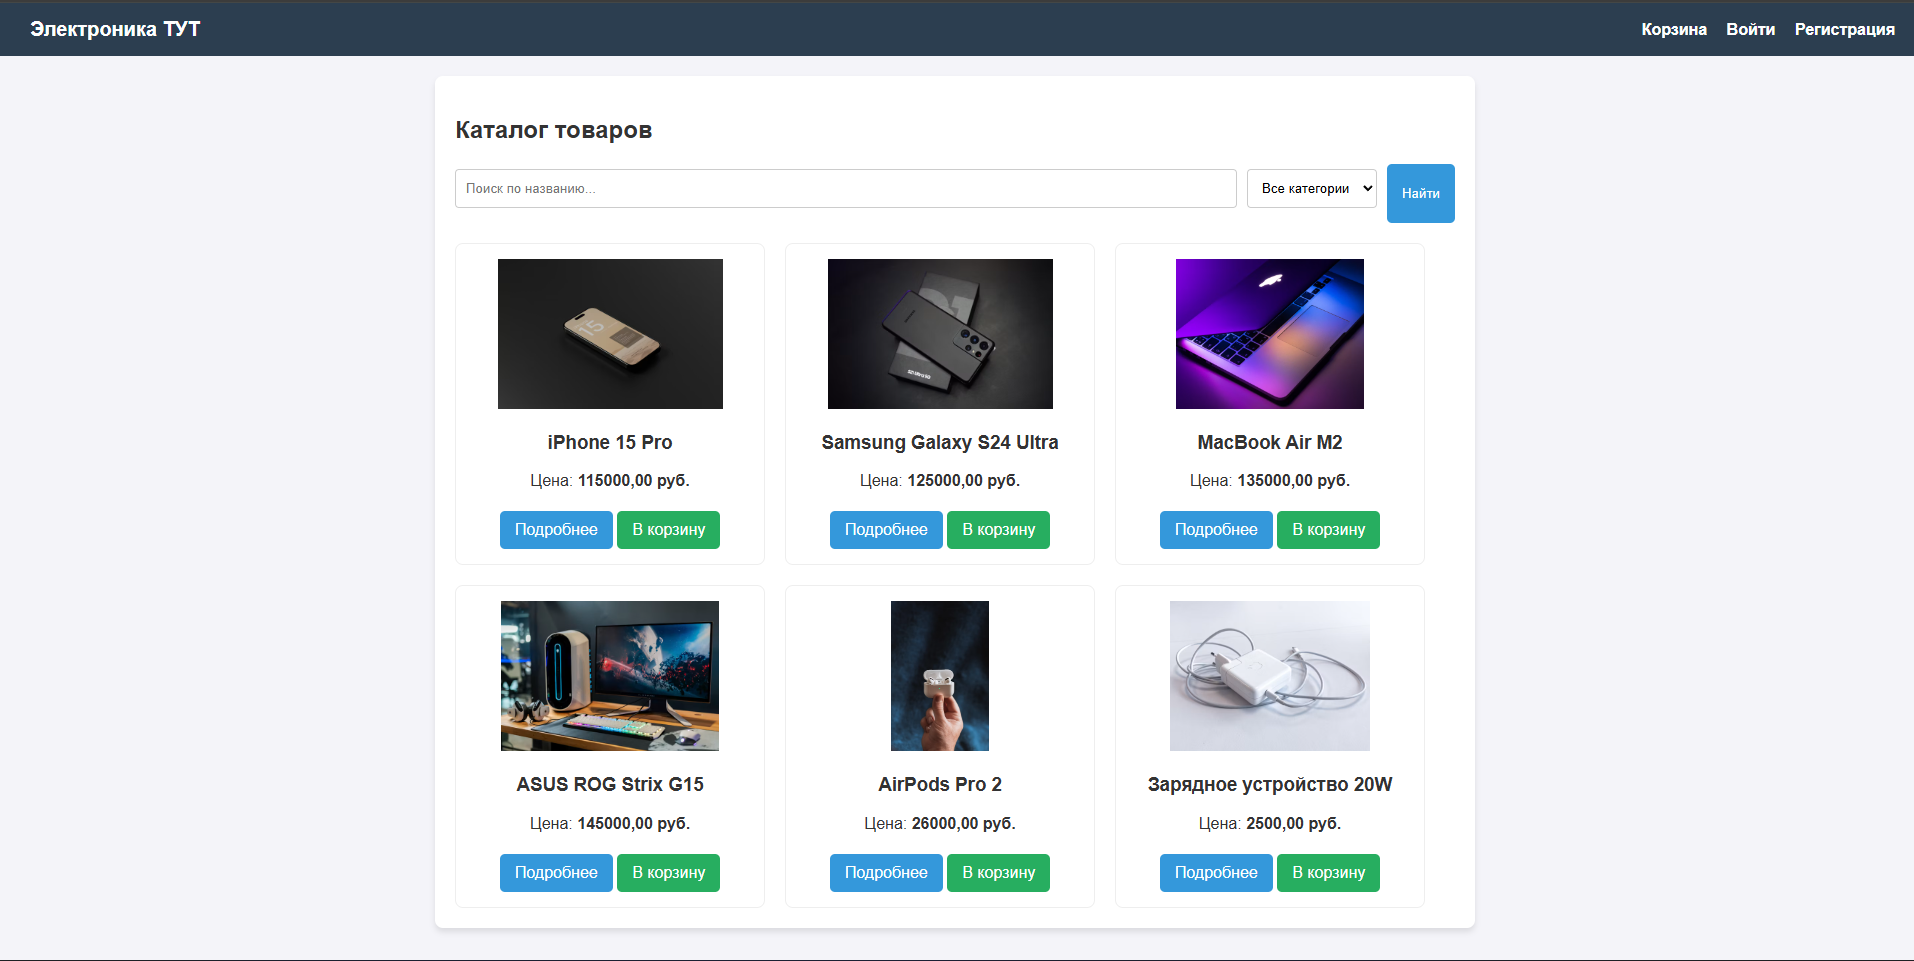
\includegraphics[width=0.95\textwidth]{images/main_website.png}
    \caption{Главная страница веб-приложения}
    \label{fig:main_website}
\end{figure}

\begin{figure}[H]
    \centering
    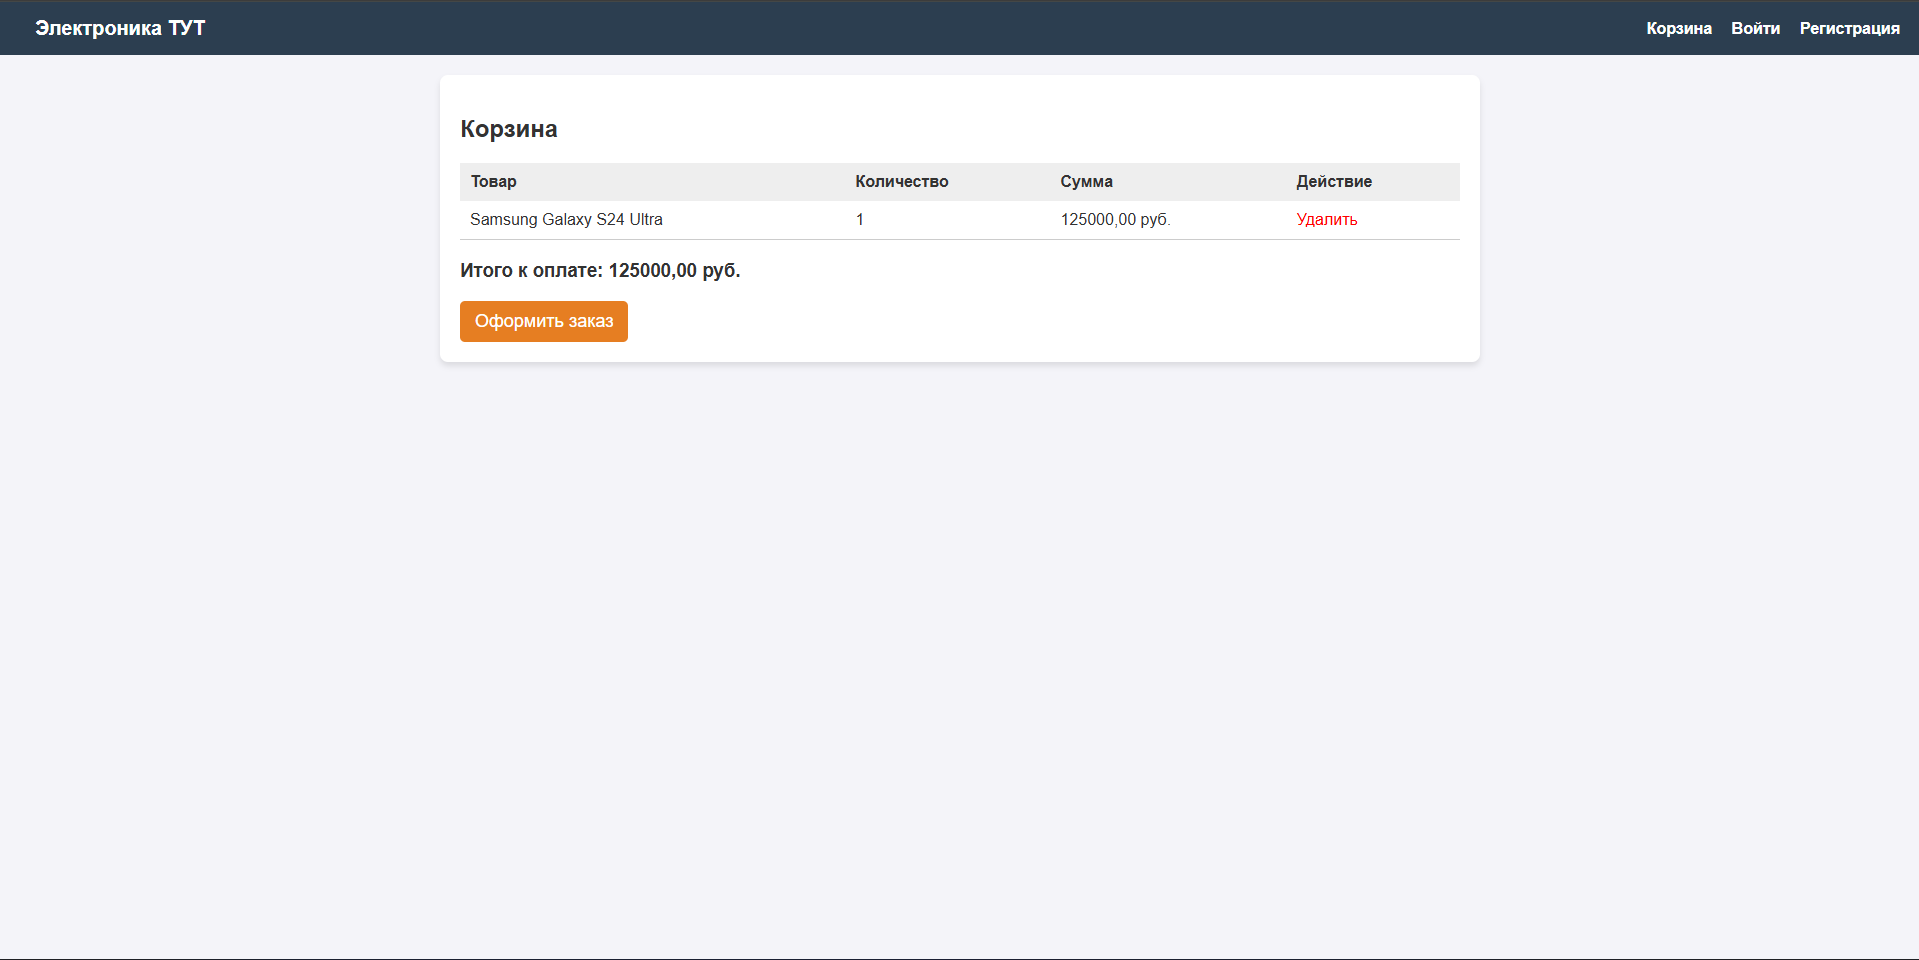
\includegraphics[width=0.95\textwidth]{images/корзина.png}
    \caption{Страница корзины пользователя}
    \label{fig:cart}
\end{figure}

Такое проектирование позволяет заранее определить состав страниц, структуру данных и
основные точки взаимодействия пользователя с системой.

\clearpage
\section*{Глава 3. Разработка веб-приложения}
\addcontentsline{toc}{section}{Глава 3. Разработка веб-приложения}
\stepcounter{section}

\subsection{Разработка базовой структуры приложения и вёрстка интерфейса}

Разработка веб-приложения была выполнена на основе фреймворка Django. Для максимальной простоты и удобства понимания весь основной функционал магазина был вынесен в одно приложение \texttt{store}. Это позволяет избежать излишней сложности и легко отслеживать связи между товарами, корзиной и заказами.

Интерфейс спроектирован с использованием базовых HTML-шаблонов и CSS (стили встроены напрямую в базовый шаблон для простоты чтения кода). Пользователю доступны главная страница с каталогом товаров, страница с детальной информацией о товаре, корзина, оформление заказа и история покупок.

\subsection{Проектирование моделей данных (товары и заказы)}

Для хранения информации в базе данных (используется стандартная база SQLite) были созданы понятные модели. Основными являются \texttt{Category} (Категория) и \texttt{Product} (Товар). 

\begin{lstlisting}[caption={Модели товаров и категорий}, language=Python]
class Category(models.Model):
    name = models.CharField(max_length=255, verbose_name="Название")
    description = models.TextField(blank=True)

class Product(models.Model):
    category = models.ForeignKey(Category, on_delete=models.CASCADE)
    name = models.CharField(max_length=255)
    description = models.TextField()
    price = models.DecimalField(max_digits=10, decimal_places=2)
    stock = models.PositiveIntegerField(default=0)
\end{lstlisting}

Связь между ними организована по принципу "один ко многим" (одна категория может содержать много товаров).

\subsection{Реализация корзины товаров}

Корзина товаров реализована наиболее простым и логичным способом — через встроенные сессии Django (\texttt{request.session}). Это значит, что корзина хранится во временной памяти сервера для каждого пользователя (даже неавторизованного) и не требует создания сложных таблиц в базе данных. В сессии хранится словарь, где ключ — это ID товара, а значение — его количество.

\begin{lstlisting}[caption={Добавление товара в корзину}, language=Python]
def add_to_cart(request, product_id):
    if 'cart' not in request.session:
        request.session['cart'] = {}
    cart = request.session['cart']
    
    product_id_str = str(product_id)
    if product_id_str in cart:
        cart[product_id_str] += 1 # увеличиваем количество
    else:
        cart[product_id_str] = 1  # добавляем новый товар
        
    request.session.modified = True
    return redirect('cart_detail')
\end{lstlisting}

\subsection{Оформление заказа и аутентификация}

Для оформления заказа пользователь должен быть авторизован. Мы использовали стандартную модель \texttt{User} из Django, что избавило от необходимости писать систему регистрации с нуля. Авторизованный покупатель может заполнить адрес, после чего содержимое его корзины из сессии переносится в базу данных в виде \texttt{Order} (Заказ) и \texttt{OrderItem} (Позиции заказа). Цены фиксируются на момент покупки.

\begin{lstlisting}[caption={Оформление заказа}, language=Python]
@login_required
def checkout(request):
    cart = request.session.get('cart', {})
    if request.method == 'POST':
        address = request.POST.get('address')
        # Создаем заказ в базе данных
        order = Order.objects.create(user=request.user, address=address)
        # Логика переноса товаров из корзины в позиции заказа...
        request.session['cart'] = {} # Очищаем корзину после заказа
        return redirect('order_history')
    return render(request, 'store/checkout.html')
\end{lstlisting}

\subsection{Реализация поиска и фильтрации товаров}

Для удобства пользователей на главной странице добавлен поиск и фильтрация. Поиск осуществляется по названию товара с использованием простого фильтра \texttt{icontains} (поиск подстроки без учета регистра), а фильтрация — по точному совпадению ID категории.

\begin{lstlisting}[caption={Поиск и фильтрация в каталоге}, language=Python]
def product_list(request):
    query = request.GET.get('q', '')
    category_id = request.GET.get('category', '')
    
    products = Product.objects.all()
    if query: # Если есть поисковый запрос
        products = products.filter(name__icontains=query)
    if category_id: # Если выбрана категория
        products = products.filter(category_id=category_id)
        
    return render(request, 'store/product_list.html', {'products': products})
\end{lstlisting}

Таким образом, веб-приложение реализует весь необходимый функционал интернет-магазина, оставаясь при этом логичным, легко читаемым и удобным для дальнейшего расширения или изучения на любительском уровне.

Исходный код разработанного веб-приложения доступен в репозитории на платформе GitHub по ссылке: \url{https://github.com/DanilaKuznetsov/coursework-web-app-main}. Доступ к репозиторию предоставлен проверяющему (GitHub: \texttt{akruzhalov}).


% Заключение
\clearpage
\section*{Заключение}
\addcontentsline{toc}{section}{Заключение}

В ходе выполнения курсовой работы была рассмотрена предметная область интернет-торговли
цифровой электроникой и определены требования к веб-приложению для управления ассортиментом
и заказами. Анализ существующих решений показал, что крупные интернет-магазины и
маркетплейсы обладают развитым функционалом, однако не всегда подходят для самостоятельного
магазина, которому требуется собственная система управления товарами, клиентами и заказами.

По результатам работы можно сформулировать следующие \textbf{выводы}:

\begin{enumerate}
    \item Для магазина цифровой электроники ключевыми функциями являются каталог с
    характеристиками товаров, поиск, фильтрация, корзина, оформление заказа и история покупок.
    \item Для серверной части проекта целесообразно использовать Django, так как он предоставляет
    встроенные средства работы с базой данных, административной панелью, пользователями и правами
    доступа.
    \item Модель данных должна учитывать связи между пользователями, категориями, товарами,
    корзиной, заказами и позициями заказа, чтобы обеспечить корректную обработку покупок.
    \item Разграничение ролей покупателей, менеджеров и администраторов повышает безопасность
    системы и упрощает организацию рабочих процессов магазина.
\end{enumerate}

\textbf{Перспективы развития проекта} связаны с добавлением онлайн-оплаты, интеграции со
службами доставки, системы отзывов, промокодов, уведомлений о статусе заказа и аналитики продаж.

При разработке пояснительной записки к курсовому проекту соблюдались требования~\cite{gost_report},
определяющие структуру и правила оформления научно-исследовательских работ.


% Список литературы
\addcontentsline{toc}{section}{Список литературы}
\begin{thebibliography}{9}
    \bibitem{django_docs}
    Django documentation. URL: \url{https://docs.djangoproject.com/} (дата обращения: 24.04.2026).

    \bibitem{flask_docs}
    Flask documentation. URL: \url{https://flask.palletsprojects.com/} (дата обращения: 24.04.2026).

    \bibitem{fastapi_docs}
    FastAPI documentation. URL: \url{https://fastapi.tiangolo.com/} (дата обращения: 24.04.2026).

    \bibitem{gost_report}
    ГОСТ 7.32-2017. Отчет о научно-исследовательской работе. Структура и правила оформления. М.: Стандартинформ, 2017.
\end{thebibliography}

% Приложения (при необходимости)
% \include{appendix}

\end{document}
